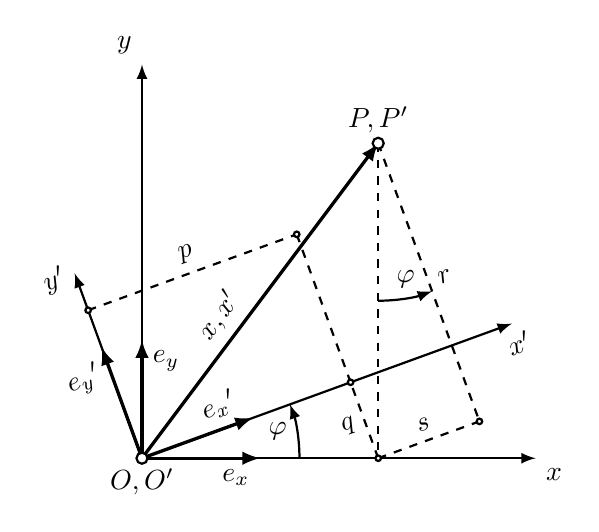
\begin{tikzpicture}
    %----------------------------------------------------------------------------------------%
    % Mathematik
    %----------------------------------------------------------------------------------------%
    \def\r{2};
    \def\u{20};
    \def\x{3};
    \def\y{4};
    \pgfmathsetmacro\xc{cos(\u)*\x};
    \pgfmathsetmacro\yc{cos(\u)*\y};
    \pgfmathsetmacro\xs{sin(\u)*\x};
    \pgfmathsetmacro\ys{sin(\u)*\y};
    %----------------------------------------------------------------------------------------%
    % Koordinaten
    %----------------------------------------------------------------------------------------%
    \coordinate (O) at (0,0);
    \coordinate (P1) at (\x,\y);
    \path (P1) -- (O-|P1) coordinate (S1);
    \path (P1) +(\u-90:\yc) coordinate (S2);
    \path (S1) +(\u+90:\xs) coordinate (S3);
    \path (S3) +(\u+90:2) coordinate (S4);
    \path (O) +(\u+90:2) coordinate (S5);
    %----------------------------------------------------------------------------------------%
    % Koordinatenachsen
    %----------------------------------------------------------------------------------------%
    \begin{scope}[thick,->,>=latex]
    \draw (O) -- +(5,0) node[anchor=north west] {$x$};
    \draw (O) -- +(0,5) node[anchor=south east] {$y$};
    \draw (O) -- +(\u:5) node[anchor=north, rotate=\u] {$x^\prime$};
    \draw (O) -- +(\u+90:2.5) node[anchor=east, rotate=\u] {$y^\prime$};
    \end{scope}
    %----------------------------------------------------------------------------------------%
    % Einheitsvektoren
    %----------------------------------------------------------------------------------------%
    \begin{scope}[very thick,->,>=latex,scale = 1.5]
    \draw (O) -- +(1,0) node[anchor = north east] {$\bvec{e_{x}}$};
    \draw (O) -- +(0,1) node[anchor = north west] {$\bvec{e_{y}}$};
    \draw (O) -- +(\u:1) node[anchor = south east,rotate=\u] {$\bvec{e_{x}}^\prime$};
    \draw (O) -- +(\u+90:1) node[anchor = north east, rotate=\u] {$\bvec{e_{y}}^\prime$};
    \end{scope}
    %----------------------------------------------------------------------------------------%
    % Vektoren
    %----------------------------------------------------------------------------------------%
    \begin{scope}[very thick,->,>=latex]
    \draw (O) -- (P1) node [midway, sloped, anchor= south east] {$\bvec{x},\bvec{x}^\prime$};
    \end{scope}
    %----------------------------------------------------------------------------------------%
    % Komponenten
    %----------------------------------------------------------------------------------------%
    \begin{scope}[thick, dashed]
    \draw (P1) -- (S1);
    \draw (P1) -- (S2) node [midway, sloped, anchor = west, rotate=90] (TextNode) {$r$};
    \draw (S1) -- (S2) node [midway, sloped, above] (TextNode) {$s$};
    \draw (S1) -- (S3) node [midway, sloped, anchor = east, rotate=90] (TextNode) {$q$};
    \draw (S5) -- (S4) node [midway, sloped, above] (TextNode) {$p$};
    \draw (S4) -- (S3);
    \end{scope}
    %----------------------------------------------------------------------------------------%
    % Punkte
    %----------------------------------------------------------------------------------------%
    \begin{scope}[thick,draw=black,fill=white]
    \filldraw (O) circle (2pt) node[anchor=north] {$O,O^\prime$};
    \filldraw (P1) circle (2pt) node[anchor=south] {$P,P^\prime$};
    \filldraw (S1) circle (1pt);
    \filldraw (S2) circle (1pt);
    \filldraw (S3) circle (1pt);
    \filldraw (S4) circle (1pt);
    \filldraw (S5) circle (1pt);
    \end{scope}
    %----------------------------------------------------------------------------------------%
    % Winkelbögen
    %----------------------------------------------------------------------------------------%
    \begin{scope}[thick,->,>=latex]
    \draw (0:\r) arc (0:\u:\r) node [midway, anchor = east] {$\varphi$};
    \draw (P1)+(0,-\r) arc (-90:\u-90:\r) node [midway, anchor = south] {$\varphi$};
    \end{scope}
    %----------------------------------------------------------------------------------------%
\end{tikzpicture}